\documentclass[conference]{IEEEtran}
\IEEEoverridecommandlockouts
% The preceding line is only needed to identify funding in the first footnote. If that is unneeded, please comment it out.
\usepackage{cite}
\usepackage{amsmath,amssymb,amsfonts}
\usepackage{algorithmic}
\usepackage{graphicx}
\usepackage{textcomp}
\usepackage{xcolor}
\usepackage{siunitx}
\usepackage{float}
\usepackage{media9}
\usepackage{subcaption}
\usepackage{minted}
\newfloat{video}{!t}{ext}
\floatname{video}{Video}
\newfloat{mylist}{!t}{ext}
\floatname{mylist}{Listing}
\def\BibTeX{{\rm B\kern-.05em{\sc i\kern-.025em b}\kern-.08em
    T\kern-.1667em\lower.7ex\hbox{E}\kern-.125emX}}

\begin{document}

\title{Self driving toy car\\
{\footnotesize Project for 3D Computer Vision lecture, summer term 2020}
}

\author{\IEEEauthorblockN{Alexander Barth}
\IEEEauthorblockA{\textit{M. Sc. student computer engineering} \\
\textit{Heidelberg University}\\
dl248@stud.uni-heidelberg.de}
\and
\IEEEauthorblockN{Grewan Hassan}
\IEEEauthorblockA{\textit{M. Sc. student physics} \\
\textit{Heidelberg University}\\
g.hassan@stud.uni-heidelberg.de}
\and
\IEEEauthorblockN{Denis Münch}
\IEEEauthorblockA{\textit{M. Sc. student applied computer science} \\
\textit{Heidelberg University}\\
denis.muench@stud.uni-heidelberg.de}
\and
\IEEEauthorblockN{Royden Wagner}
\IEEEauthorblockA{\textit{M. Sc. student computer engineering} \\
\textit{Heidelberg University}\\
royden-wagner@outlook.com}
}

\maketitle

\begin{abstract}
This report describes the self driving car toy project done in the 3D Computer Vision lecture at Heidelberg University.
The goal is to train neural networks so that the given car can drive autonomously on a track.
\end{abstract}

\begin{IEEEkeywords}
autonomous driving, computer vision, image processing, neural networks
\end{IEEEkeywords}

\section{Getting started}
For getting started an operating system needs to be flashed onto the Raspberry Pi 3 B+ which is mounted into the car.
Through the Raspberry Pi Imager the Pi OS 32-bit in release 2020-05-27 was flashed onto the SD card.
The OS is a port of Debian with the Raspberry Pi Desktop and comes with an integrated configurator to enable SSH, VNC, the camera, SPI and I2C.
During our project several different approaches are used.
Roughly divided into an approach with and without machine learning.
The first approach is classical image processing without machine learning by using OpenCV.

\section{Image Processing without ML}\label{sec:no_ml}

The goal of this approach is to let the car drive autonomously on the track without using machine learning.
Therefore the approach can be roughly divided into two subtasks, the image processing with OpenCV and the driving.
OpenCV is an open library for computer vision and machine learning of which the first part is used.


\subsection{Driving} \label{ssec:drive}

Once again the driving task can be divided into the following two subtasks, steering and throttle.
The Raspberry is mounted on the vehicle together with a servo and an Arduino PCA9685 controller.
The donkeycar application is steering through the PCA9685.
This can be observed while following the donkeycar user guide in the step of calibrating the car.
Calibrating the donkeycar takes the plugged in channel and the bus, which are the same required options using the \textit{Adafruit\_9685} library.
Every time the calibrate function is executed a new donkeycar instance is initiated.
Therefore our driving function writes directly to the controller without the donkeycar instance.
Nevertheless the donkeycar calibrate function is helpful for getting the PWM values at which the steering is full left, straight and full right.
Using the other channel the same procedure can be used to get the PWM values for full throttle, zero and full throttle backwards.
Table \ref{tab:pwmval} shows the different PWM values observed while using the calibrate function.

\begin{table}[!t]
	\renewcommand{\arraystretch}{1.3}
	\caption{PWM values}
	\centering
	\begin{tabular}{r|l}
		mode&value\\
		\hline
		left & 460\\
		center & 380\\
		right & 290\\
		forwards & 500\\
		stop & 370\\
		backwards & 220\\
	\end{tabular}
	\label{tab:pwmval}
\end{table}

By using the boundary values each with the null value a respective linear equation can be set up.
\begin{description}[\IEEEsetlabelwidth{Backwards}]
\setlength\itemsep{.25em}
\item[Left] $ pulse\_length = -4.4 * angle + 380 $
\item[Right] $ pulse\_length = -3.6 * angle + 380 $
\item[Forwards] $ pulse\_length = 1.4 * acceleration + 360 $
\item[Backwards] $ pulse\_length = 0.6 * acceleration + 360 $
\end{description}
These resulting equations are used in \textit{driving\_functions.py}.
It can be used for steering and controlling the motor directly and is later used inside the python script for autonomous driving.
The input for the steering function are steering angles reaching from \numrange{-25}{25} which are converted into degrees and into PWM signals.
Using steering angles is easier for the human because they do not need to be abstracted.
Similiar way is used for the motor control.
Input values to the motor control function are percentages of the acceleration reaching from \numrange{-100}{100} which are again converted into PWM signals.

\subsection{Lane Detection} \label{ssec:lanedet}

Second subtask for driving autonomously is to detect the track lanes.
The result is shown in Figure \ref{fig:lanedet}.
Figure \ref{sub:frame} shows the input frame which is processed by the python script.
A ROI (region of interest) is extracted from the input frame.
The stencil is the filled version of the ROI frame.
In Figure \ref{sub:frame} the colors are used as follows:
\begin{description}[\IEEEsetlabelwidth{Yellow}]
	\setlength\itemsep{.25em}
	\item[Green] Left lane arrays.
	\item[Red] Mean value of the left lane arrays.
	\item[Blue] Right lane arrays.
	\item[Pink] Mean value of the right lane arrays.
	\item[Yellow] Direction where to go. The lower point is located at the center of the image edge. The upper point is the center between the distant points of both lanes. This is only the case while both lanes are detected. Is only one lane detected the upper point of the yellow line is at the endpoint of the edge moved by a quarter of the picture width. This is estimated the half of the track width
\end{description}

\begin{figure*}[t]
	\centering
	\begin{subfigure}[c]{0.24\textwidth}
		\centerline{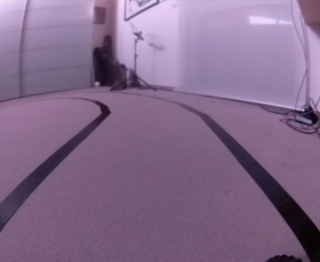
\includegraphics[height=3cm]{media/lane_frame}}
		\subcaption{Lane frame.}
		\label{sub:lane}
	\end{subfigure}
	\begin{subfigure}[c]{0.24\textwidth}
		\centerline{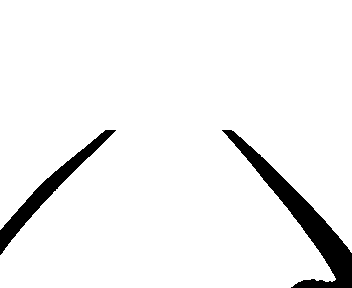
\includegraphics[height=3cm]{media/roi_frame}}
		\subcaption{ROI frame.}
		\label{sub:roi}
	\end{subfigure}
	\begin{subfigure}[c]{0.24\textwidth}
		\centerline{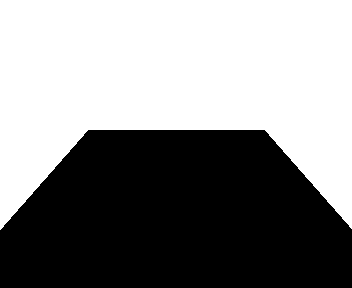
\includegraphics[height=3cm]{media/stencil}}
		\subcaption{Stencil.}
		\label{sub:stencil}
	\end{subfigure}
	\begin{subfigure}[c]{0.24\textwidth}
		\centerline{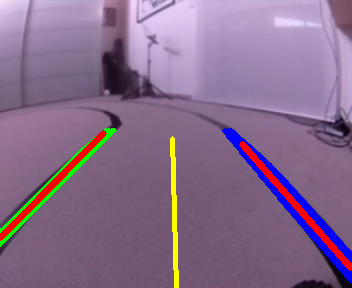
\includegraphics[height=3cm]{media/frame}}
		\subcaption{Frame.}
		\label{sub:frame}
	\end{subfigure}
	\caption{Lane detection.}
	\label{fig:lanedet}
\end{figure*}

This is done by using the Hough line transformation \cite{Hough1962}.
Normally edge detection is part of the algorithm.
In other words the edge image is crucial as input.
In our case an edge detection algorithm like Canny is redundant.
This is first because of the simplicity of our input frames.
Second the ROI frame which is inputted into the Hough line transformation is inverted because the ROI frame is black on white while most edge detection outputs are white on black.
By inverting it the resulting input to the transformation is close to edge images.
The other input parameters for the python HoughLinesP function are theta, threshold, minLineLength and maxLaneGap.
\begin{description}[\IEEEsetlabelwidth{minLineLength}]
	\setlength\itemsep{.25em}
	\item[minLineLength] The minimum line length is needed so that only the track edges are detected and processed as lanes. If the value is too low the edge of the right front wheel is detected which can be clearly seen in Figure \ref{sub:lane} and \ref{sub:roi}. 
	\item[maxLineGap] This describes the distance between the endpoints of both lanes at the picture center and is estimated.
\end{description}

The P function ending indicates that the probabilistic Hough line transform is applied instead of the standard version.
It is a more efficient implementation which has a different output, the extremes of the detected lines.
Instead of only the function it is helpful to understand how the Hough line transform works.
The description $y = mx + c$ is not always the best way to describe a line.
Therefore the hessian normalform is used resulting in the parametric equation $d = x * \cos \alpha + y * \sin \alpha$.
The algorithm detects lines described by this equation in the given input.
Also a helper function was used to distinguish lines marking left and right lanes.
Since the Hough line transformation algorithm walks column-wise through the image from the left top to the right bottom the helper function splits right and left.
The left lane is completely detected and finished before the area of the image where the right lane is located is processed by the algorithm.

\subsection{Autonomous Driving}

Both subtasks merged together result in autonomous driving.
Video \ref{vid:autodrive} shows a short extract from driving.

\begin{video}[h]
	\includemedia[
	width=0.9\linewidth,
	height=0.5\linewidth,
	addresource=media/steering.mp4,
	transparent, %transparent player background
	deactivate=onclick,
	activate=onclick,
	flashvars={source=media/steering.mp4
		&hideBar=false
		&autoplay=true
		&loop=true % loop video
		&controlBarMode=floating
		&controlBarAutoHide=false
		&scaleMode=letterbox % preserve aspect ratio while scaling the video
	}
	]{}{VPlayer.swf}
	\caption{Direction and steering angle while driving.}
	\label{vid:autodrive}
	\centering
\end{video}

The video also contains the steering angle values which are also indicated by the yellow direction line as shown in Figure \ref{sub:frame}.
The autonomous driving script contains the helper function to calculate the direction which was already explained in Section \ref{ssec:lanedet}.
If no lane is detected the direction for steering is straight ahead.
Another helper function calculates the steering angle from the desired direction which can be used afterwards as the input for the steering command described in Section \ref{ssec:drive}.
To minimize the error rate of the steering angle a helper function stabilizes the angle by comparing it to the previous calculated values.
This is useful since the direction differs a lot if only one lane is detected correctly.
Video \ref{vid:datacrtl} contains some of these errors.
While steering left the direction aims a few times to the right lane because as explained before the direction is pointing towards the endpoint of the edge moved by a quarter of the picture width while the left lane is not detected correctly.

\begin{video}[h]
	\includemedia[
	width=0.9\linewidth,
	height=0.5\linewidth,
	addresource=media/dataset_ctrl.mp4,
	transparent, %transparent player background
	deactivate=onclick,
	activate=onclick,
	flashvars={source=media/dataset_ctrl.mp4
		&hideBar=false
		&autoplay=true
		&loop=true % loop video
		&controlBarMode=floating
		&controlBarAutoHide=false
		&scaleMode=letterbox % preserve aspect ratio while scaling the video
	}
	]{}{VPlayer.swf}
	\caption{Dataset with control values.}
	\label{vid:datacrtl}
	\centering
\end{video}

Video \ref{vid:uturn} shows the car driving a turn from external view.

\begin{video}[h]
	\includemedia[
	width=0.9\linewidth,
	height=0.5\linewidth,
	addresource=media/uturn.mp4,
	transparent, %transparent player background
	deactivate=onclick,
	activate=onclick,
	flashvars={source=media/uturn.mp4
		&hideBar=false
		&autoplay=true
		&loop=true % loop video
		&controlBarMode=floating
		&controlBarAutoHide=false
		&scaleMode=letterbox % preserve aspect ratio while scaling the video
	}
	]{}{VPlayer.swf}
	\caption{Driving a turn from external view.}
	\label{vid:uturn}
	\centering
\end{video}

The overall benefit from this approach will be discussed in the next subsection.
As seen in the videos own tracks were used for testing which is a result of the pandemic situation and the distribution of all team members.
Some other problems result from the hardware built into the car.
The occasionally has a red color cast which sometimes disappears.
Controlling the throttle through the Arduino controller did not always affect the output to the wheels.
The wheel speed was very high and did not correlate to the linear equations put into the driving functions script.
Below 18\% the vehicle did not drive at all, above the speed was too high.
Therefore a turtle driving mode was created and is shown in Listing \ref{lst:turtle}.

\begin{mylist}[h]
\begin{minted}[breaklines,linenos,fontsize=\footnotesize,breaksymbolindent=0pt]{python}
def turtle_mode():
 try:
  pwm = config_pwm(hz=60)
  lane_detection_proc = multiprocessing.Process(target=main, args=())
  lane_detection_proc.start()
  time.sleep(1)
  motor_proc = multiprocessing.Process(target=go_slow_multistep, args=(pwm, 22, 0.15, 2,))
  motor_proc.start()
 except KeyboardInterrupt:
  lane_detection_proc.terminate()
  lane_detection_proc.join()

  motor_proc.terminate()
  motor_proc.join()

  motor_ctrl(0, pwm)
  steering(0, pwm)
\end{minted}
\caption{Turtle mode function for driving.}
\label{lst:turtle}
\end{mylist}

The turtle driving mode is also a great possibility for creating datasets.
Since the car is driving slowly more and better data can be recorded.

\subsection{Benefit}

It may be unclear what the benefit from an approach without machine learning might be.
Therefore this will now be clarified.
The approach is completely detached from donkeycar.
Steering and motor are controlled directly through the Arduino PCA controller.
Also the code is from scratch in latest versions.
This is a great benefit for future work with the car in a teaching environment.
Process thinking regarding driving is detached from donkeycar and also machine learning approaches in future work can be done completely without it what marks a difference to our machine learning approaches.
Also it clarifies which components are built in the car.
This might be unclear since receiving an already built car pushes to box thinking without being aware of the connection between parts or the presence and function of the Arduino controller.

\textbf{•TODO:} (Decorator, Dataclass, "`sugaring"')

\section{Donkeycar Autopilot}

Although we decided against using the donkeycar library in its entirety for the reasons stated in subsection \ref{ssec:drive}, we did experiment with it in an OpenAI gym environment called gym-donkeycar, which simulates a car that a donkeycar application can run on.

Donkeycar 2.5.8 comes with the ability to collect data and train a neural network built-in.

\subsection{Data Collection}

At each step the gym environment returns the image that the virtual car sees. 
The steering angle and throttle value are passed to the gym as a numpy array of length two by the donkeycar application. 
When recording drive footage, \textit{json} files containing an image file name, steering angle, throttle value and other miscellaneous information are saved with the associated images in a folder. 
These folders can be used to train a model.

\subsection{Training}

Different model types are available under the \textit{donkeycar.parts.keras module}.
As the name indicates these model types are built with the Keras API on top of TensorFlow.
The available types are:
\begin{description}[\IEEEsetlabelwidth{Categorical}]
\setlength\itemsep{.25em}
\item[Categorical] takes an image as input and and has two categorical outputs for steering and throttle. The input is passed to a network with the following layers:
\begin{enumerate}
\item
5x5 Conv-ReLU, 24 filters, stride 2
\item
5x5 Conv-ReLU, 32 filters, stride 2
\item
5x5 Conv-ReLU, 64 filters, stride 2 or 3x3 Conv-ReLU, 64 filters, stride 1
\item
3x3 Conv-ReLU with 64 filters and stride 2 or 3x3 Conv-ReLU, 64 filters, stride 1
\item
3x3 Conv-ReLU, 64 filters, stride 1
\item
Dense-ReLU, 100 outputs
\item
Dense-ReLU, 50 outputs
\item
Dense-Softmax, 15 outputs for steering and Dense-Softmax, 20 outputs for throttle
\end{enumerate}
\item[Linear] takes an image as input and has two scalar outputs for steering and throttle. The input is passed to a network with the following layers:
\begin{enumerate}
\item
5x5 Conv-ReLU, 24 filters, stride 2
\item
5x5 Conv-ReLU, 32 filters, stride 2
\item
5x5 Conv-ReLU, 64 filters, stride 2
\item
3x3 Conv-ReLU, 64 filters, stride 1
\item
3x3 Conv-ReLU, 64 filters, stride 1
\item
Dense-ReLU, 100 outputs
\item
Dense-ReLU, 50 outputs
\item
Dense-Linear, 1 output for steering and Dense-Linear, 1 output for throttle
\end{enumerate}
\item[IMU] takes an image and an inertial measurement unit vector as input and has two scalar outputs for steering and throttle. The image is passed to a Linear network without layers 7 and 8, while the IMU vector is passed to a network with 3 Dense-ReLU layers with 14 outputs each. The outputs of both networks are concatenated and passed to a network with 2 Dense-ReLU layers with 50 outputs each and two separate Dense-Linear layers with 1 output for steering and throttle respectively.
\item[Latent] takes an image as input and has two scalar outputs and an image output. This experimental model type uses convolutional layers to learn a latent vector and transposed convolutional layers to reconstruct an image from the latent vector as well as dense layers to produce the steering and throttle outputs from the same latent vector.
\item[RNN] takes a sequence of images as input and has one 2D output for steering and throttle. The images are passed to a Linear network whose last Conv-ReLU layer is replaced with a 2x2 MaxPooling layer and the Dense-ReLU layer with 50 outputs is removed entirely. To make use of the sequence of images, each layer is wrapped inside a TimeDistributed layer, which applies the wrapped layers to each input. Two Long Short-Term Memory layers with 128 outputs followed by four Dense-ReLU layers with 128, 64, 10, and 2 outputs respectively complete the network.
\item[3D] takes a sequence of images as input and has one 2D output for steering and throttle. The input is passed to a network with the following layers:
\begin{enumerate}
\item
3x3x3 3D Conv-ReLU, 16 filters, stride (1,3,3)
\item
1x2x2 3D MaxPooling, stride (1,2,2)
\item
3x3x3 3D Conv-ReLU, 32 filters, stride (1,1,1)
\item
1x2x2 MaxPooling, stride (1,2,2)
\item
3x3x3 3D Conv-ReLU, 64 filters, stride (1,1,1)
\item
1x2x2 3D MaxPooling, stride (1,2,2)
\item
3x3x3 3D Conv-ReLU, 128 filters, stride (1,1,1)
\item
1x2x2 3D MaxPooling, stride (1,2,2)
\item
Dense-BatchNorm-ReLU, 256 outputs
\item
Dense-BatchNorm-ReLU, 256 outputs
\item
Dense, 2 outputs
\end{enumerate}
\item[Behaviour] takes an image and a behaviour vector as input and has two categorical outputs. The image is passed to a Linear network without layers 7 and 8, while the Behaviour vector is passed to a network with 3 Dense-ReLU layers with each layers outputs twice its inputs. The outputs of both networks are concatenated and passed to a network with a Dense-ReLU layers with 100 outputs followed by one with 50 outputs and two separate Dense-Linear layers with 15 outputs for steering and 20 outputs for throttle.
\item[Localizer] takes an image as input and has two scalar outputs for steering and throttle and one categorical output for location. The image is passed to a Linear network which has an additional Dense-ReLU output layer for a location output with the number of outputs specified by the user.
\end{description}

\subsection{Results}

We recorded five laps worth of footage, i.e., images and associated steering angles and throttle values, on the track ``donkey-generated-track-v0'' and trained five models on the data. The model types used were: 3D, Categorical, Latent, Linear, and RNN. Behaviour, IMU, and Localizer couldn't be used due to technical constraints of the gym-environment. We let the model drive the car for 50 laps and measured the distance travelled by the model driver if the car veered off track before completing the 50 laps. The 3D model type was the only one incapable of following the track. Recommended models are Linear for a smooth driving experience and Categorical if speed is more important than smoothness.

\begin{table}[!t]
\renewcommand{\arraystretch}{1.3}
\caption{Simulation Results}
\centering
\begin{tabular}{rll}
type&laps&fastest lap\\
\hline
3D&-&-\\
Categorical&50&24s\\
Latent&50&31s\\
Linear&50&29s\\
RNN&50&32s\\
\end{tabular}
\label{tab:simresults}
\end{table}

\section{DAgger}

\subsection{Description}

DA\textsc{gger} (Dataset Aggregation), developed by Ross et al. \cite{Ross2011}, is an iterative algorithm, which in each iteration \( i \) uses policy \( \pi_i \) to collect in dataset \( \mathcal{D}_i \) state-action pairs \( (s,\pi^*(s)) \), where \( s \) is the state visited by the policy \( \pi_i \) and \( \pi^*(s) \) is the associated action returned by an expert policy \( \pi^* \). A classifier \( \hat{ \pi}_{i+1} \) is then trained on \( \mathcal{D} = \mathcal{D}_1 \cup \dotsm \cup \mathcal{D}_i \) (see Figure \ref{fig:dagger}).

In practice this means an expert, in our case \textbf{•TODO:} (lane follower), takes control of the autonomous car and collects image-action pairs, where the action is a steering angle and a throttle value. A classifier is trained on the available data and used to collect new images, all of which are then labeled by the expert. Those new image-action pairs are combined with the old and used to train the next classifier. The process of data collection, expert labelling, and training is repeated until a satisfactory classifier has been trained.

\begin{figure}[h]
\begin{algorithmic}[1]
\STATE Initialize \(\mathcal{D}\gets \emptyset\)
\FOR{ \( i=1 \) \TO \( N \)}
\STATE Let \( \pi_i = \beta_i \pi^* + \left( 1- \beta_i\right)\hat{ \pi}_i \).
\STATE Sample \textit{T}-step trajectories using \( \pi_i \).
\STATE Get dataset \( \mathcal{D}_i = \left\{ \left( s, \pi^*(s)\right)\right\} \) of visited states by \( \pi_i \) and actions given by expert.
\STATE Aggregate datasets: \( \mathcal{D}\gets \mathcal{D} \cup \mathcal{D}_i \).
\STATE Train classifier \( \hat{ \pi}_{i+1} \) on \( \mathcal{D} \).
\ENDFOR
\RETURN best \( \hat{ \pi}_i \) on validation.
\end{algorithmic}
\caption{DA\textsc{gger} algorithm}
\label{fig:dagger}
\end{figure}

Note, that due to the lack of data and therefore policies in the first iteration, we usually set
\[
\beta_i = \begin{cases}
1,\quad\text{if }i=1\\
0,\quad\text{else}
\end{cases}
\]
or
\[
\beta_i = \begin{cases}
1,\quad\text{if }i=1\\
p^{i-1},\quad\text{else}
\end{cases}
\]
where \( p \) is some probability, to directly utilize the expert as our first policy. Subsequent policies \( \hat{ \pi}_{i+1} \) are trained on expert labeled states visited by the current policy \( \pi_i \) or a combination of the current policy and the expert policy.

\subsection{Implementation}
We used a neural network, implemented in PyTorch, similar to the Linear network used by donkeycar to train the next policy on the expert labeled dataset. For details on the expert implementation see section \ref{sec:no_ml}. We set \( \beta_1 = 1 \) utilizing the expert in the first iteration and \( \beta_{2:n} = 0 \) utilizing the trained policy in the remaining iterations.

\subsection{Results}
We measure distance travelled by the trained policy until the car veers off track. See table \ref{tab:results} for results.

\begin{table}[!t]
\renewcommand{\arraystretch}{1.3}
\caption{Results}
\centering
\begin{tabular}{r|l}
iteration&distance travelled\\
\hline
1&x laps\\
\end{tabular}
\label{tab:results}
\end{table}

\section{Conclusion}

\section{Placeholder}

move to best fitting (sub-)section

\begin{video}[!t]
	\includemedia[
	width=0.9\linewidth,
	height=0.5\linewidth,
	addresource=media/dataset.mp4,
	transparent, %transparent player background
	deactivate=onclick,
	activate=onclick,
	flashvars={source=media/dataset.mp4
		&hideBar=false
		&autoplay=true
		&loop=true % loop video
		&controlBarMode=floating
		&controlBarAutoHide=false
		&scaleMode=letterbox % preserve aspect ratio while scaling the video
	}
	]{}{VPlayer.swf}
	\caption{Dataset.}
	\label{vid:dataset}
\end{video}

\begin{video}[!t]
	\includemedia[
	width=0.9\linewidth,
	height=0.5\linewidth,
	addresource=media/model.mp4,
	transparent, %transparent player background
	deactivate=onclick,
	activate=onclick,
	flashvars={source=media/model.mp4
		&hideBar=false
		&autoplay=true
		&loop=true % loop video
		&controlBarMode=floating
		&controlBarAutoHide=false
		&scaleMode=letterbox % preserve aspect ratio while scaling the video
	}
	]{}{VPlayer.swf}
	\caption{Model driving in simulation.}
	\label{vid:model}
\end{video}

\begin{thebibliography}{00}
	
\bibitem{Abadi2016} M. Abadi et al. ``Tensorflow: Large-scale machine learning on heterogeneous distributed systems,'' arXiv preprint, 2016.
\bibitem{Hough1962} P. Hough. ``Method and means for recognizing complex patterns'', United States Patent Office, 3069654, 1962
\bibitem{Leavers1992} V. Leavers. ``Shape Detection in Computer Vision Using Hough Transform'', Springer, London, UK, 1992
\bibitem{Ross2011} S. Ross et al. ``A Reduction of Imitation Learning and Structured Prediction to No-Regret Online Learning'', Proceedings of the Fourteenth International Conference on Artificial Intelligence and Statistics, {AISTATS} 2011, Fort Lauderdale, USA, April 11-13, 2011
\end{thebibliography}

\end{document}
